\citeauthor{Zhao2014} present an interactive visual analysis system designed for revealing and analyzing anomalies spreading in social media. The main challenge of system is to distill valuabe information from streamed social media data, due to the heterogeneous and dynamic crowd behaviours \iacite{Zhao2014}. The challenge is not further described in this thesis because it is irrelevant as related work. However, some parts of the visual analysis system are very interesting and worth a rough analysis.

Figure \ref{fig:fluxflow} on page \pageref{fig:fluxflow} shows FluxFlow. It is based on multiple views combined with linking and brushing. As one can see, it deconstructs heterogeneous social media data and builds some kind of tree. The tree can be navigated and single nodes can be highlighted with hovering. Clicking on a single node creates a new view showing all its subnodes as circles on a timeline. The radius of the circle depends on an attribute of the data item. The creation of the timeline is linear animated. Each click on a node appends a new timeline in given view.

\begin{figure}[!htb]
\centering
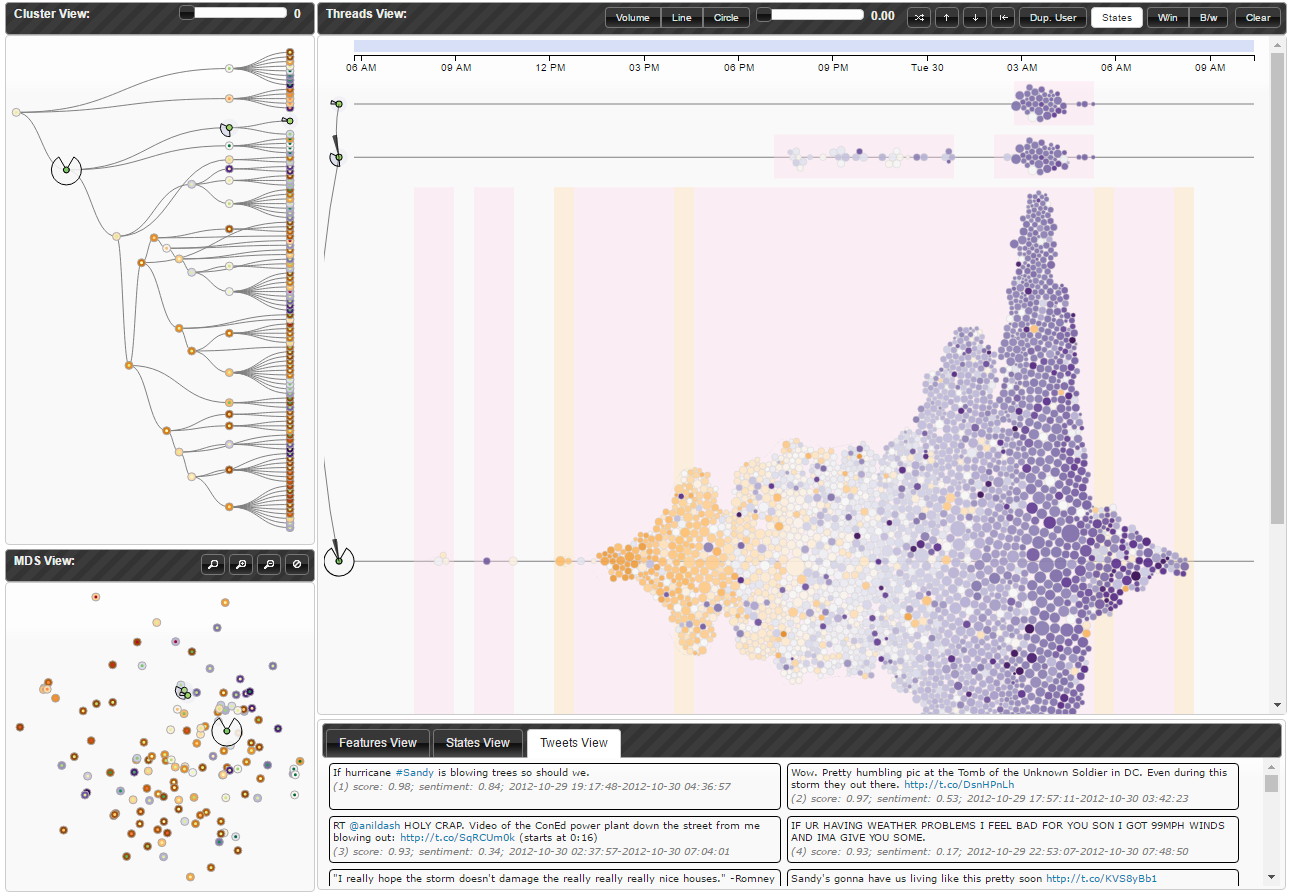
\includegraphics[height=5cm]{images/methods/related/fluxflow.png}
\caption[
    Fluxflow: a visual analysis system \iacite{Zhao2014}.
]{Fluxflow: a visual analysis system}
\label{fig:fluxflow}
\end{figure}

The use case of such a system is very well described in the paper, therefore making it easy to analyze possible datasets. Even though the main challenge of the system is to analyze streamed data, the visualization itself is only based on static datasets. It is not clear if the system is able to build the tree from a table dataset itself or if the tree must be given.
The objective of FluxFlow is to show anomalies in social media data and discover insights with using the multiple view system combined with multiple visual channels and interaction methods. Manipulating the visualization is possible through interaction with the timeline, selecting interesting nodes in the tree or entering specific time slots to view.